% Diagram: V9.0 Convergence Cascade --- Real Data
% 8 islands: 4 Basin A, 2 Basin B, 2 outliers (all briefly hit 44.52 kg)
% Data extracted from convergence_history.csv using Julia
\documentclass{article}
\usepackage{tikz}
\usepackage[paperwidth=34cm,paperheight=23cm,margin=0.5cm]{geometry}
\pagestyle{empty}

\begin{document}
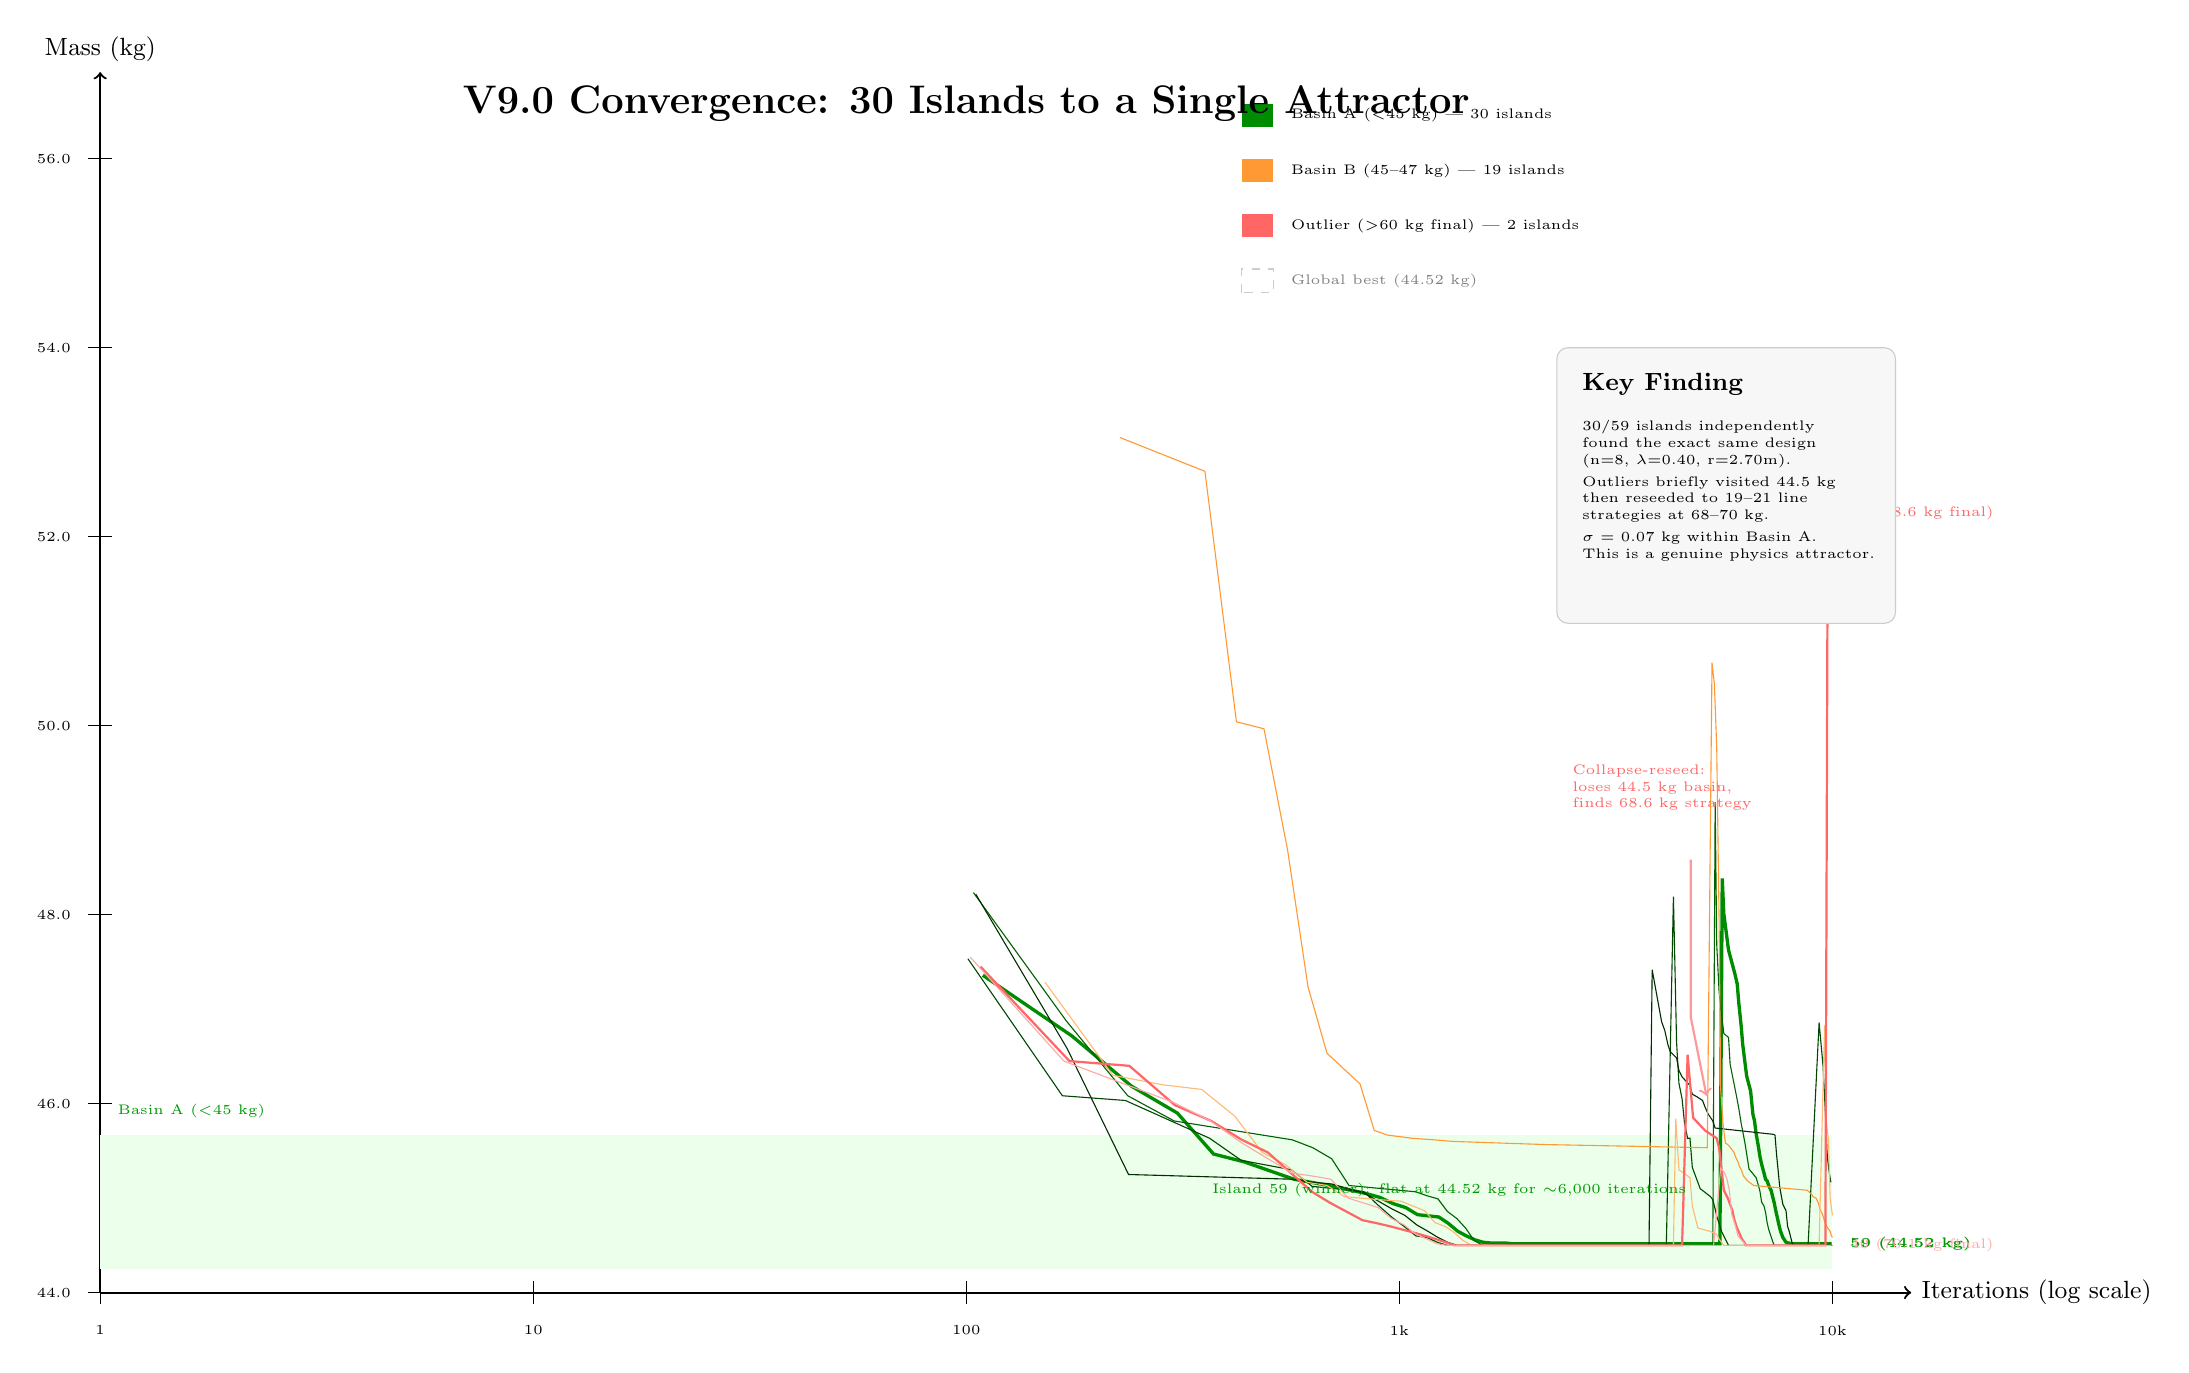
\begin{tikzpicture}[scale=1.0]

% Coordinate mapping:
%   x = log10(iteration) * 5.5  (range: 0 to 22 = 1 to 10,000 iterations)
%   y = (mass_kg - 44.0) * 1.2  (range: 44 to 56 kg)

% Axes
\draw[->, thick] (0,0) -- (0,15.5) node[above] {\small Mass (kg)};
\draw[->, thick] (0,0) -- (23,0) node[right] {\small Iterations (log scale)};

% X ticks
\foreach \x/\lab in {0.0/1, 5.5/10, 11.0/100, 16.5/1k, 22.0/10k}{
  \draw (\x,-0.15) -- (\x,0.15);
  \node[below, font=\tiny] at (\x,-0.3) {\lab};
}

% Y ticks
\foreach \y/\lab in {0.0/44.0, 2.4/46.0, 4.8/48.0, 7.2/50.0, 9.6/52.0, 12.0/54.0, 14.4/56.0}{
  \draw (-0.15,\y) -- (0.15,\y);
  \node[left, font=\tiny] at (-0.25,\y) {\lab};
}

% 44.52 kg guide line
\draw[gray!40, dashed] (0,0.624) -- (22,0.624);
\node[font=\tiny, gray!60, anchor=south east] at (22,0.624) {44.52 kg};

% Basin A convergence zone highlight
\fill[green!8] (0,0.3) rectangle (22,2.0);
\node[font=\tiny, green!60!black, anchor=south west] at (0.1,2.1) {Basin A ($<$45 kg)};

% ── Island 59 (winner, Basin A) ──
% Real data: starts ~94 kg, converges to 44.52 at iter ~1000, flat thereafter
% Truncated above 56 kg, spike points annotated
\draw[green!55!black, very thick] plot coordinates {
(11.21,4.03) (12.34,3.26) (13.10,2.62) (13.68,2.28) (14.14,1.76) (14.53,1.66)
(15.16,1.44) (15.66,1.35) (16.07,1.26) (16.25,1.21) (16.42,1.13) (16.58,1.08)
(16.73,0.99) (17.00,0.96) (17.12,0.88) (17.24,0.78) (17.35,0.72) (17.46,0.67)
(17.56,0.64) (17.66,0.63) (17.76,0.63) (17.85,0.63) (17.94,0.62) (18.02,0.62)
(18.10,0.62) (18.18,0.62) (18.33,0.62) (18.48,0.62) (18.67,0.62) (18.86,0.62)
(19.08,0.62) (19.38,0.62) (19.73,0.62) (20.14,0.62) (20.57,0.62) (20.60,5.26)
(20.62,4.81) (20.68,4.35) (20.76,4.05) (20.79,3.92) (20.81,3.68) (20.84,3.39)
(20.86,3.15) (20.91,2.75) (20.96,2.56) (20.99,2.26) (21.01,2.18) (21.03,2.02)
(21.06,1.85) (21.08,1.72) (21.10,1.63) (21.13,1.52) (21.15,1.44) (21.17,1.42)
(21.19,1.36) (21.22,1.30) (21.24,1.22) (21.26,1.14) (21.28,1.04) (21.30,0.95)
(21.32,0.86) (21.34,0.78) (21.37,0.70) (21.39,0.67) (21.41,0.64) (21.43,0.63)
(21.45,0.63) (21.47,0.62) (21.50,0.62) (21.52,0.62) (21.56,0.62) (21.60,0.62)
(21.66,0.62) (21.73,0.62) (21.81,0.62) (21.90,0.62) (21.99,0.62)
};
\node[font=\tiny\bfseries, green!60!black, anchor=west] at (22.1,0.62) {59 (44.52 kg)};

% ── Island 4 ──
\draw[green!38!black, thin] plot coordinates {
(11.09,5.08) (12.27,3.45) (13.05,2.50) (13.64,2.18) (15.14,1.94) (15.40,1.84)
(15.64,1.70) (15.86,1.36) (16.71,1.28) (16.85,1.23) (16.99,1.19) (17.11,1.03)
(17.23,0.94) (17.34,0.82) (17.45,0.66) (17.56,0.60) (17.66,0.60) (17.75,0.60)
(17.84,0.60) (18.02,0.60) (18.18,0.60) (18.40,0.60) (18.67,0.60) (18.97,0.60)
(19.33,0.60) (19.73,0.60) (20.21,0.60) (20.48,0.60) (20.51,6.23) (20.53,4.42)
(20.56,3.82) (20.62,3.29) (20.68,3.24) (20.70,2.90) (20.76,2.60) (20.78,2.50)
(20.81,2.34) (20.84,2.15) (20.86,2.05) (20.89,1.89) (20.94,1.57) (21.03,1.46)
(21.06,1.36) (21.08,1.28) (21.10,1.15) (21.13,1.10) (21.15,1.02) (21.17,0.89)
(21.19,0.80) (21.21,0.74) (21.24,0.65) (21.26,0.60) (21.28,0.60) (21.32,0.60)
(21.38,0.60) (21.46,0.60) (21.56,0.60) (21.66,0.60) (21.78,0.60) (21.90,0.60)
(21.99,0.60)
};

% ── Island 21 ──
\draw[green!28!black, thin] plot coordinates {
(11.02,4.24) (12.22,2.50) (13.02,2.44) (14.09,1.96) (14.49,1.68) (15.13,1.56)
(15.39,1.35) (16.05,1.28) (16.23,1.11) (16.40,0.96) (16.56,0.84) (16.71,0.72)
(16.85,0.70) (16.98,0.64) (17.11,0.60) (17.23,0.60) (17.45,0.60) (17.75,0.60)
(18.09,0.60) (18.47,0.60) (18.91,0.60) (19.38,0.60) (19.89,0.60) (19.98,5.03)
(20.02,3.18) (20.05,2.66) (20.09,2.46) (20.12,2.16) (20.16,1.96) (20.19,1.96)
(20.22,1.59) (20.32,1.32) (20.45,1.22) (20.48,1.18) (20.51,1.06) (20.53,0.97)
(20.56,0.88) (20.59,0.78) (20.62,0.72) (20.65,0.66) (20.68,0.60) (20.73,0.60)
(20.81,0.60) (20.91,0.60) (21.03,0.60) (21.17,0.60) (21.34,0.60) (21.52,0.60)
(21.69,0.60) (21.83,3.43) (21.88,2.88) (21.91,2.28) (21.93,1.80) (21.94,1.68)
(21.96,1.52) (21.98,1.40)
};

% ── Island 35 ──
\draw[green!18!black, thin] plot coordinates {
(11.12,5.06) (12.28,3.10) (13.06,1.50) (15.14,1.44) (15.41,1.40) (15.64,1.38)
(16.06,1.26) (16.41,1.06) (16.57,0.98) (16.72,0.86) (16.86,0.78) (16.99,0.70)
(17.11,0.64) (17.23,0.60) (17.35,0.60) (17.56,0.60) (17.84,0.60) (18.18,0.60)
(18.61,0.60) (19.08,0.60) (19.67,0.60) (19.71,4.10) (19.83,3.44) (19.87,3.33)
(19.91,3.15) (19.94,3.06) (20.02,2.98) (20.05,2.82) (20.09,2.74) (20.19,2.63)
(20.22,2.52) (20.29,2.48) (20.35,2.44) (20.38,2.36) (20.42,2.27) (20.48,2.18)
(20.51,2.09) (21.25,2.01) (21.27,2.00) (21.29,1.75) (21.31,1.55) (21.33,1.34)
(21.37,1.12) (21.41,1.04) (21.43,0.84) (21.45,0.78) (21.47,0.70) (21.49,0.62)
(21.51,0.60) (21.55,0.60) (21.59,0.60) (21.64,0.60) (21.71,0.60) (21.80,0.60)
(21.92,0.60) (22.00,0.60)
};

% ── Island 15 (Basin B, converged slower to 45.0) ──
\draw[orange!80, thin] plot coordinates {
(12.95,10.86) (14.03,10.43) (14.43,7.25) (14.78,7.16) (15.08,5.62) (15.34,3.88)
(15.58,3.04) (16.00,2.65) (16.18,2.06) (16.35,2.00) (16.51,1.98) (16.66,1.96)
(16.80,1.95) (16.94,1.94) (17.18,1.92) (18.36,1.88) (20.41,1.84) (20.47,8.00)
(20.50,7.73) (20.53,6.92) (20.56,4.72) (20.58,2.59) (20.61,2.14) (20.64,1.90)
(20.67,1.88) (20.69,1.86) (20.72,1.82) (20.75,1.78) (20.77,1.72) (20.80,1.66)
(20.82,1.60) (20.85,1.54) (20.87,1.48) (20.92,1.42) (21.00,1.36) (21.68,1.30)
(21.72,1.26) (21.74,1.24) (21.75,1.22) (21.79,1.20) (21.82,1.14) (21.84,1.06)
(21.85,1.04) (21.87,1.00) (21.89,0.94) (21.90,0.90) (21.92,0.86) (21.94,0.82)
(21.97,0.78) (21.98,0.74) (22.00,0.70)
};

% ── Island 38 (Basin B, found 44.52 then reseeded) ──
\draw[orange!55, thin] plot coordinates {
(12.00,3.94) (12.86,2.76) (13.49,2.64) (13.99,2.58) (14.41,2.24) (14.76,1.78)
(15.06,1.62) (15.33,1.40) (15.58,1.36) (15.80,1.22) (16.00,1.20) (16.52,1.16)
(16.67,1.10) (16.82,1.04) (16.95,0.89) (17.08,0.84) (17.20,0.76) (17.31,0.66)
(17.42,0.60) (17.53,0.60) (17.72,0.60) (17.99,0.60) (18.31,0.60) (18.72,0.60)
(19.17,0.60) (19.72,0.60) (19.98,0.60) (20.01,2.21) (20.05,1.56) (20.19,1.46)
(20.22,1.10) (20.29,0.82) (20.44,0.78) (20.53,0.74) (20.56,0.68) (20.59,0.64)
(20.62,0.60) (20.65,0.60) (20.70,0.60) (20.78,0.60) (20.88,0.60) (21.01,0.60)
(21.17,0.60) (21.38,0.60) (21.63,0.60) (21.83,0.60) (21.90,3.40) (21.92,2.20)
(21.93,2.10) (21.95,1.93) (21.97,1.20) (22.00,0.98)
};

% ── Island 11 (OUTLIER --- found 44.52, reseeded to 68.6 kg) ──
\draw[red!60, thick] plot coordinates {
(11.18,4.14) (12.31,2.94) (13.07,2.88) (13.65,2.38) (14.11,2.18) (14.50,1.94)
(14.83,1.78) (15.39,1.28) (15.62,1.14) (16.03,0.92) (16.22,0.88) (16.39,0.84)
(16.54,0.80) (16.69,0.76) (16.83,0.72) (16.96,0.68) (17.09,0.64) (17.20,0.60)
(17.32,0.60) (17.43,0.60) (17.63,0.60) (17.90,0.60) (18.22,0.60) (18.64,0.60)
(19.15,0.60) (19.74,0.60) (20.09,0.60) (20.16,3.02) (20.23,2.22) (20.38,2.06)
(20.53,1.96) (20.56,1.84) (20.59,1.58) (20.62,1.30) (20.64,1.26) (20.67,1.20)
(20.70,1.12) (20.73,1.04) (20.75,0.94) (20.78,0.84) (20.85,0.68) (20.88,0.64)
(20.90,0.60) (20.93,0.60) (21.00,0.60) (21.09,0.60) (21.20,0.60) (21.35,0.60)
(21.55,0.60) (21.78,0.60) (21.89,0.60) (21.91,0.60) (21.94,9.90) (21.97,9.78)
};
\node[font=\tiny, red!60, anchor=west] at (22.1,9.90) {11 (68.6 kg final)};

% ── Island 40 (OUTLIER --- found 44.52, reseeded to 70.1 kg) ──
\draw[red!35, thin] plot coordinates {
(11.05,4.26) (12.24,2.94) (13.03,2.64) (13.62,2.42) (14.10,2.18) (14.50,1.90)
(14.83,1.70) (15.13,1.52) (15.40,1.48) (15.63,1.44) (15.85,1.20) (16.23,1.08)
(16.40,0.94) (16.56,0.86) (16.71,0.74) (16.85,0.68) (16.98,0.62) (17.11,0.60)
(17.34,0.60) (17.65,0.60) (18.01,0.60) (18.47,0.60) (19.02,0.60) (19.69,0.60)
(20.37,0.60) (20.49,0.60) (20.58,1.58) (20.63,1.52) (20.66,1.44) (20.69,1.30)
(20.72,1.00) (20.77,0.84) (20.80,0.72) (20.87,0.64) (20.90,0.60) (20.95,0.60)
(21.02,0.60) (21.11,0.60) (21.23,0.60) (21.39,0.60) (21.57,0.60) (21.77,0.60)
(21.94,0.60) (21.99,0.60)
};
\node[font=\tiny, red!35, anchor=west] at (22.1,0.60) {40 (70.1 kg final)};

% ── Annotations ──
% Reseed spike callout for Island 11
\draw[red!40, ->, thick] (20.2, 5.5) -- (20.2, 3.5) -- (20.4, 2.5);
\node[font=\tiny, red!60, text width=3cm, align=left, anchor=south] at (20.2, 6.0) {
  Collapse-reseed:\\
  loses 44.5 kg basin,\\
  finds 68.6 kg strategy};

% Island 59 label
\node[font=\tiny, anchor=west, green!60!black] at (14.0, 1.3) {Island 59 (winner): flat at 44.52 kg for $\sim$6,000 iterations};

% Legend
\fill[green!55!black] (14.5, 14.8) rectangle (14.9, 15.1);
\node[font=\tiny, anchor=west] at (15.0, 14.95) {Basin A ($<$45 kg) --- 30 islands};
\fill[orange!80] (14.5, 14.1) rectangle (14.9, 14.4);
\node[font=\tiny, anchor=west] at (15.0, 14.25) {Basin B (45--47 kg) --- 19 islands};
\fill[red!60] (14.5, 13.4) rectangle (14.9, 13.7);
\node[font=\tiny, anchor=west] at (15.0, 13.55) {Outlier ($>$60 kg final) --- 2 islands};
\draw[gray!40, dashed] (14.5, 12.7) rectangle (14.9, 13.0);
\node[font=\tiny, anchor=west, gray] at (15.0, 12.85) {Global best (44.52 kg)};

% Title
\node[font=\Large\bfseries] at (11, 15.1) {V9.0 Convergence: 30 Islands to a Single Attractor};

% Findings box
\fill[black!3, draw=gray!40, rounded corners=4pt] (18.5, 8.5) rectangle (22.8, 12.0);
\node[font=\small\bfseries, anchor=north west] at (18.7, 11.8) {Key Finding};
\node[font=\tiny, text width=3.8cm, align=left, anchor=north west] at (18.7, 11.2) {
30/59 islands independently\\found the exact same design\\(n=8, $\lambda$=0.40, r=2.70m).\\[2pt]
Outliers briefly visited 44.5 kg\\then reseeded to 19--21 line\\strategies at 68--70 kg.\\[2pt]
$\sigma$ = 0.07 kg within Basin A.\\This is a genuine physics attractor.
};

\end{tikzpicture}
\end{document}
